
\documentclass{mise_en_page}
\usepackage[utf8]{inputenc}
\usepackage[T1]{fontenc}
\usepackage[french]{babel}
\usepackage{amsmath}
\usepackage{amssymb,amsfonts,textcomp}
\usepackage{array}
\usepackage{supertabular}
\usepackage{hhline}

\makeatletter
\newcommand\arraybslash{\let\\\@arraycr}
\makeatother
\setlength\tabcolsep{1mm}
\renewcommand\arraystretch{1.3}

\projet{Projet Ingéniérie}
\equipe{H4314}
\responsable{Tristan Delizy}
\redacteurs{Arnaud Lahache} % Optionnel
\titre{Best Practice 2 : Aide à la rédaction d’un CdC Logiciel}
\version{1.3}
\objet{Ce dossier a pour but de définir les règles de bonnes pratiques dans le
cadre de la rédaction d’un cahier des charges logiciel  devant intégrer
le système documentaire dans le cadre du projet COPEVUE-MONIT}
\etat{validé} %draft, non relu, non validé, validé

\begin{document}

\maketitle

\begin{historique}
    \histo{1.0}{16/01/2012}{Draft initial}
    \histo{1.1}{23/01/2012}{Évolution du document}
    \histo{1.2}{30/01/2012}{Finalisation}
    \histo{1.3}{30/01/2012}{Validation}
\end{historique}

\newpage

\tableofcontents

\section[Définitions]{Définitions}
Un cahier des charges sert de base à la rédaction des clauses
contractuelles techniques, de qualité et des réception à partir
desquelles le réalisateur proposera les spécifications fonctionnelles
du logiciel.

Les objectifs d{\textquotesingle}un cahier des charges logiciel sont :

\begin{itemize}
\item préciser les orientations et le champ du domaine étudié,
\item analyser l{\textquotesingle}existant au niveau organisation,
documents utilisés, traitements effectués, données manipulées,
\item proposer des solutions d{\textquotesingle}organisation,
fonctionnelles et techniques répondant aux exigences et besoins
exprimés,
\item obtenir une description globale du système (organisationnelle,
fonctionnelle, technique, contraintes majeures de sécurité, de
performance, interfaces avec d{\textquotesingle}autres systèmes, ...),
\item vérifier la faisabilité organisationnelle et technique,
\item aboutir à un choix argumenté d{\textquotesingle}une solution type
de développement.
\end{itemize}


\section[Documents de référence]{Documents de référence}
GLOSSAIRE / Glossaire

QUALITE / Gestion de la documentation

\section[Méthodologie de rédaction]{Méthodologie de
rédaction}


\subsection[Processus d’élaboration du cahier des
charges]{Processus d’élaboration du cahier des charges}

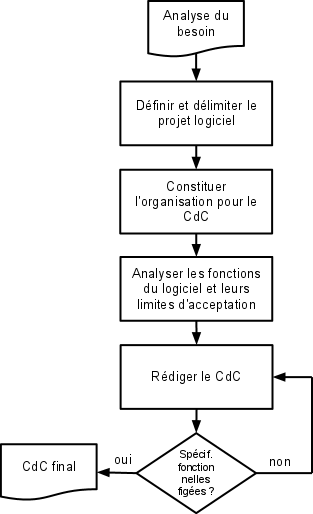
\includegraphics[width=8.308cm,height=13.6cm]{BP22020Aide20C3A020la20rC3A9daction20dun20CdC20Logiciel-img1.png}

\subsection[Etablissement d’un cahier des charges et choix d’un
fournisseur]{Etablissement d’un cahier des charges et choix
d’un fournisseur}



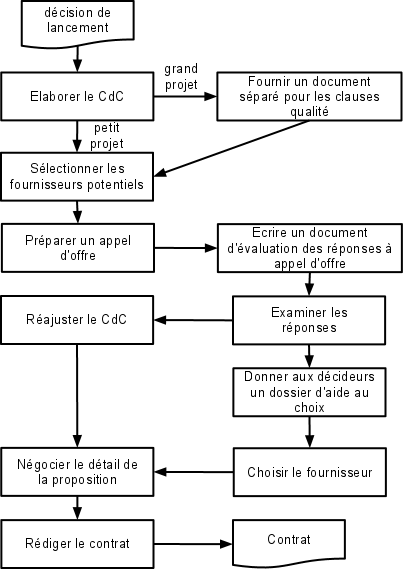
\includegraphics[width=10.663cm,height=15.081cm]{BP22020Aide20C3A020la20rC3A9daction20dun20CdC20Logiciel-img2.png}




\section[Contenu d’un Cahier des Charges]{Contenu d’un
Cahier des Charges}
\subsection[Plan Type]{4.1. Plan Type}


\begin{flushleft}
\tablehead{}
\begin{supertabular}{|m{16.345cm}|}
\hline
1. Introduction

1.1. Présentation du projet

1.2. Présentation du document

1.3. Documents applicables / Documents de référence

1.4. Terminologie et abréviations

2. Présentation du problème

2.1. Use cases (utilisateurs concernés ; But ; Nature du logiciel)

2.2. Formulation des besoins (généraux), exploitation et ergonomie,
expérience

2.3. Portée, développement, mise en oeuvre, organisation de la
maintenance

3. Exigences fonctionnelles

3.1. Fonctions de bases, performances et aptitudes

3.2. Contraintes d’utilisation

3.3. Critères d’appréciation de la réalisation effective de la fonction

3.4. Flexibilité dans la façon de mettre en oeuvre la fonction
concernée, variation de coûts associée en fonction de cette flexibilité

4. Exigences non fonctionnelles

5. Contraintes imposées, faisabilité technologique et éventuellement
moyens

5.1. Sûreté, planning, organisation, communication

5.2. Complexité

5.3. Compétences, moyens et règles

5.4. Normes de documentation

6. Configuration cible

6.1. Matériel et logiciels

6.2. Stabilité de la configuration

7. Grille d’évaluation

8. Annexes

8.1. Observations de l’existant

8.2. Proposition d’orientation

8.3. Image(s) d’écran(s) principal(aux) du logiciel

8.4. Résultat de l’analyse de la valeur

8.5. Description des API avec reste du système

(8.6. Choix d’une solution et justifications)

(8.7. Appréciation de la solution retenue)\\\hline
\end{supertabular}
\end{flushleft}


\subsection[Introduction]{Introduction}
Cette partie a pour but de présenter le projet / logiciel, ainsi que de
préciser les documents de références nécessaires à la bonne
compréhension du document.

\subsection[Présentation du problème]{Présentation du problème}
Expression des besoins à satisfaire pour le logiciel :

\begin{itemize}
\item but et principes du logiciel
\item Besoins, exploitation et ergonomie, expérience
\item Portée, développement mise en oeuvre, organisation de la
maintenance
\item Limites du projet
\end{itemize}

\subsection[Exigences fonctionnelles]{Exigences fonctionnelles}
Propriétés spécifiques du logiciel, cycle de vie et modèles
organisationnels des traitements et des données qu’il contient.

Les fonctionnalités sont triées par ordre de priorité : plus une
fonction est importante et critique pour le logiciel, plus cette
fonction est placée vers le haut.

Exemple d’un tableau descriptif d’une fonctionnalité :

\begin{flushleft}
\tablehead{}
\begin{supertabular}{|m{3.8219998cm}|m{12.324cm}|}
\hline
N° Fonctionnalité &
0\\\hline
Nom &
{\textless}Nom de la fonctionnalité{\textgreater}\\\hline
Description &
{\textless}Description complète de la fonction
désirée{\textgreater}\\\hline
Performances &
{\textless}Performance désirée{\textgreater}\\\hline
Contraintes d’utilisation &
{\textless}Spécifier ici les contraintes liées à l’utilisation de la
fonction{\textgreater}\\\hline
\end{supertabular}
\end{flushleft}

\subsection[Exigences non fonctionnelles]{4.4. Exigences non
fonctionnelles}
Il s’agit ici de décrire les exigences non fonctionnelles du logiciel.
Il s’agit de choisir les critères non fonctionnels (ERGONOMIE,
FIABILITÉ, …) nécessaires pour satisfaire les besoins non fonctionnels
utilisateurs.

\subsection[Contraintes imposées]{Contraintes imposées}
Environnement du développement du logiciel nécessaire à son élaboration 
:

\begin{itemize}
\item Organisation nécessaire pour le développement (phases de
développement, planning, délais, tests)
\item Complexité du produit logiciel (volume des données, nouveauté,
technologies nécessaires)
\item La compétence, la dimension et l’environnement de l’équipe de
développement (langage, outils, moyens)
\end{itemize}

\subsection[Configuration cible]{Configuration cible}
Concerne le matériel et les logiciels à utiliser :

\begin{itemize}
\item Description de l’environnement opérationnel
\item Stabilité
\item Contraintes d’exploitation, règlementation
\item Interfaces logiciel / matériel, IHM, BDD, API
\end{itemize}


\subsection[Grille d’évaluation]{Grille d’évaluation}
Evaluation de la description des fonctions proposées par le réalisateur
par rapport aux fonctions de base du logiciel.\newline

Exemple de grille d’évaluation :

\begin{flushleft}
\tablehead{}
\begin{supertabular}{|m{3.9279997cm}|m{3.9279997cm}|m{3.9279997cm}|m{3.963cm}|}
\hline
\centering Critères {\textbackslash} Fonctions &
\centering F1 &
\centering F2 &
\centering\arraybslash ...\\\hline
\centering Indication des amendements ou variantes proposées &
\centering Evaluation de la fonction en fonction du critère &
\centering ... &
\centering\arraybslash ...\\\hline
\centering Justification des options et modalités de contrôle &
\centering ... &
\centering ... &
~
\\\hline
\centering Prix du logiciel et de ses options &
\centering ... &
~
 &
~
\\\hline
\centering Mesures prises pour respecter les contraintes, conséquences &
~
 &
~
 &
~
\\\hline
\centering Coût d’installation, d’exploitation, maintenance &
~
 &
~
 &
~
\\\hline
\centering Décomposition du logiciel en composants et coût de
réalisation &
~
 &
~
 &
~
\\\hline
\centering Prévision de fiabilité &
~
 &
~
 &
~
\\\hline
\centering Espérance de vie du logiciel en fonction des évolutions
technologiques &
~
 &
~
 &
~
\\\hline
\end{supertabular}
\end{flushleft}

\section[Gestion du document]{Gestion du document}


Le document de type {\textless}{\textless}Cahier des
Charges{\textgreater}{\textgreater} doit respecter les éléments de
gestion de la documentation énoncés dans le dossier QUALITE / Gestion
de la documentation.
\end{document}
